%% ============================================================
%%  Leader-Follower Multi-Robot System — Student Assignment
%%  Model-Driven Engineering (MDE) Lab
%%  Compile: pdflatex student_assignment.tex  (twice for refs)
%% ============================================================
\documentclass[11pt, a4paper]{article}

%% --- Encoding / Fonts ---
\usepackage[T1]{fontenc}
\usepackage[utf8]{inputenc}
\usepackage{lmodern}
\usepackage{microtype}

%% --- Page layout ---
\usepackage[top=2.5cm, bottom=2.5cm, left=2.8cm, right=2.8cm]{geometry}

%% --- Math ---
\usepackage{amsmath, amssymb}

%% --- Colour (must come before tikz so dvipsnames are available to pgf/tikz) ---
\usepackage[dvipsnames]{xcolor}

%% --- Graphics ---
\usepackage{graphicx}
\usepackage{tikz}
\usetikzlibrary{automata, positioning, arrows.meta, shapes.geometric, fit, backgrounds, calc}

\definecolor{mdeblue}{RGB}{30,90,160}
\definecolor{mdegray}{RGB}{240,242,246}
\definecolor{mdegreen}{RGB}{20,140,60}
\definecolor{mdeorange}{RGB}{210,100,0}
\definecolor{mdered}{RGB}{190,30,30}
\definecolor{taskbg}{RGB}{255,250,235}
\definecolor{taskborder}{RGB}{200,150,0}
\definecolor{infobg}{RGB}{235,245,255}
\definecolor{infoborder}{RGB}{60,120,200}
\definecolor{warnbg}{RGB}{255,240,235}
\definecolor{warnborder}{RGB}{200,80,30}
\definecolor{codebg}{RGB}{248,248,248}
\definecolor{mdepurple}{RGB}{100,30,160}

%% --- Boxes ---
\usepackage{tcolorbox}
\tcbuselibrary{breakable, skins, listings}

%% Task box
\newtcolorbox{taskbox}[2][]{
  colback=taskbg, colframe=taskborder,
  fonttitle=\bfseries\sffamily,
  title={#2},
  breakable, #1
}
%% Info box
\newtcolorbox{infobox}[2][]{
  colback=infobg, colframe=infoborder,
  fonttitle=\bfseries\sffamily,
  title={#2},
  breakable, #1
}
%% Warning box
\newtcolorbox{warnbox}[2][]{
  colback=warnbg, colframe=warnborder,
  fonttitle=\bfseries\sffamily,
  title={#2},
  breakable, #1
}

%% --- Code listings ---
\usepackage{listings}
\lstdefinestyle{pycode}{
  language=Python,
  backgroundcolor=\color{codebg},
  basicstyle=\ttfamily\footnotesize,
  keywordstyle=\color{mdeblue}\bfseries,
  stringstyle=\color{mdegreen},
  commentstyle=\color{gray}\itshape,
  numberstyle=\tiny\color{gray},
  numbers=left, stepnumber=1,
  frame=single, framerule=0.4pt,
  breaklines=true, breakatwhitespace=true,
  showstringspaces=false,
  tabsize=4
}
\lstdefinestyle{xmlcode}{
  language=XML,
  backgroundcolor=\color{codebg},
  basicstyle=\ttfamily\footnotesize,
  keywordstyle=\color{mdeblue}\bfseries,
  stringstyle=\color{mdegreen},
  commentstyle=\color{gray}\itshape,
  frame=single, framerule=0.4pt,
  breaklines=true,
  showstringspaces=false,
  tabsize=2
}
\lstdefinestyle{shellcode}{
  backgroundcolor=\color{black!92},
  basicstyle=\ttfamily\footnotesize\color{white},
  keywordstyle=\color{cyan}\bfseries,
  stringstyle=\color{green!60!white},
  commentstyle=\color{gray!60}\itshape,
  morecomment=[l]{\#},
  frame=none,
  breaklines=true,
  showstringspaces=false,
  morekeywords={export,source,ros2,colcon,launch,run,topic,node,bag,
                echo,list,info,record,kill,awk,mkdir,cd,grep}
}
\lstdefinestyle{uppaalcode}{
  backgroundcolor=\color{codebg},
  basicstyle=\ttfamily\footnotesize,
  keywordstyle=\color{mdepurple}\bfseries,
  commentstyle=\color{gray}\itshape,
  morecomment=[l]{//},
  frame=single, framerule=0.4pt,
  breaklines=true,
  showstringspaces=false,
  morekeywords={chan, broadcast, clock, int, bool, process,
                state, init, trans, guard, sync, update,
                system, A, E, not, deadlock, imply, and, or}
}

%% --- Tables ---
\usepackage{booktabs}
\usepackage{tabularx}
\usepackage{multirow}
\usepackage{array}

%% --- Lists ---
\usepackage{enumitem}
\setlist[itemize]{leftmargin=1.5em}
\setlist[enumerate]{leftmargin=1.5em}

%% --- Section title style (load before hyperref) ---
\usepackage{titlesec}
\titleformat{\section}[block]
  {\Large\bfseries\sffamily\color{mdeblue}}
  {\thesection}{1em}{}[\titlerule]
\titleformat{\subsection}[block]
  {\large\bfseries\sffamily\color{mdeblue!80}}
  {\thesubsection}{1em}{}
\titleformat{\subsubsection}[block]
  {\normalsize\bfseries\sffamily\color{mdeblue!60}}
  {\thesubsubsection}{1em}{}

%% --- Headers / Footers ---
\usepackage{fancyhdr}
\pagestyle{fancy}
\fancyhf{}
\fancyhead[L]{\small\sffamily MDE Lab — Leader-Follower Multi-Robot System}
\fancyhead[R]{\small\sffamily\thepage}
\fancyfoot[C]{\small\sffamily\color{gray}ROS2 Humble · Gazebo Classic · Uppaal 5.x}
\renewcommand{\headrulewidth}{0.4pt}

%% --- Hyperlinks ---
\usepackage{hyperref}
\hypersetup{
  colorlinks=true,
  linkcolor=mdeblue,
  citecolor=mdegreen,
  urlcolor=mdeorange,
  pdftitle={MDE Lab: Leader-Follower Multi-Robot System},
  pdfauthor={MDE Lab}
}

%% --- Misc ---
\usepackage{parskip}
\usepackage{caption}
\usepackage{subcaption}
\usepackage{float}
\usepackage{pifont}   % for \ding symbols
\newcommand{\cmark}{\textcolor{mdegreen}{\ding{51}}}
\newcommand{\xmark}{\textcolor{mdered}{\ding{55}}}

%% Counter for exercises
\newcounter{exercise}[section]
\renewcommand{\theexercise}{\thesection.\arabic{exercise}}

\newenvironment{Ex}[1]
  {\refstepcounter{exercise}\begin{taskbox}{Exercise \theexercise\ --- #1}}
  {\end{taskbox}}

%% ============================================================
\begin{document}
%% ============================================================

%% ────────────────────────────────────────────────────────────
%%  TITLE PAGE
%% ────────────────────────────────────────────────────────────
\begin{titlepage}
\centering
\vspace*{2cm}

{\Huge\bfseries\sffamily\color{mdeblue}
  Model-Driven Engineering Lab\\[0.4em]
  \Large Leader-Follower Multi-Robot System\\[0.2em]
  \normalsize with ROS2, Gazebo, and Uppaal
}

\vspace{1.5cm}
\rule{0.6\textwidth}{1.5pt}
\vspace{1.5cm}

\begin{center}
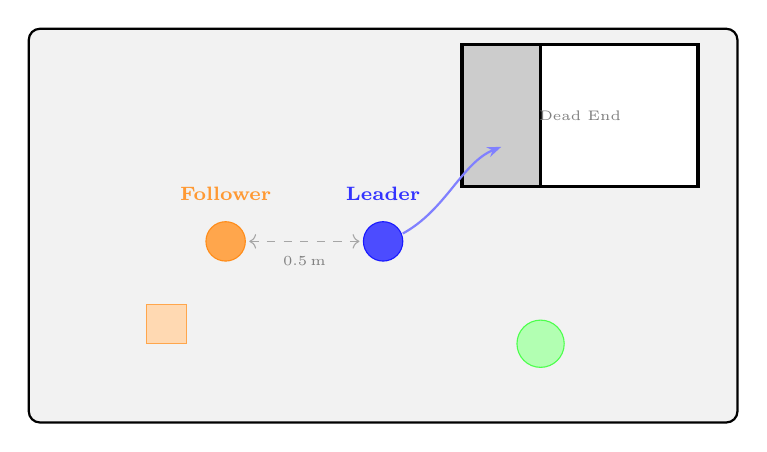
\begin{tikzpicture}[scale=1.0]
  %% Simple diagram of two robots and a map
  \draw[thick, fill=gray!10, rounded corners=4pt] (-4.5,-2.5) rectangle (4.5,2.5);
  %% Dead-end corridor
  \draw[very thick, fill=gray!40] (1.0,0.5) rectangle (4.0,2.3);
  \draw[very thick, fill=white] (2.0,0.5) rectangle (4.0,2.3);
  \draw[very thick] (1.0,0.5) -- (1.0,2.3) -- (4.0,2.3) -- (4.0,0.5);
  \node[font=\tiny, gray] at (2.5,1.4) {Dead End};
  %% Obstacles
  \filldraw[fill=orange!30, draw=orange!70] (-3.0,-1.5) rectangle (-2.5,-1.0);
  \filldraw[fill=green!30, draw=green!70] (2.0,-1.5) circle (0.3);
  %% Leader robot
  \filldraw[fill=blue!70, draw=blue!90] (0.0,-0.2) circle (0.25);
  \node[font=\scriptsize\bfseries, blue!80, above=4pt] at (0.0,0.05) {Leader};
  %% Follower robot
  \filldraw[fill=orange!70, draw=orange!90] (-2.0,-0.2) circle (0.25);
  \node[font=\scriptsize\bfseries, orange!80, above=4pt] at (-2.0,0.05) {Follower};
  %% Arrow between (below the robots to avoid overlap)
  \draw[<->, dashed, gray!70] (-1.7,-0.2) -- (-0.3,-0.2);
  \node[font=\tiny, gray, below=2pt] at (-1.0,-0.2) {0.5\,m};
  %% Connection line to dead end
  \draw[-{Stealth[length=5pt]}, blue!50, thick] (0.25,-0.1) .. controls (0.8,0.2) and (1.0,0.8) .. (1.5,1.0);
\end{tikzpicture}
\end{center}

\vspace{1.0cm}
\rule{0.6\textwidth}{1.5pt}
\vspace{1.0cm}

\large
\begin{tabular}{ll}
\textbf{Course:}     & Model-Driven Engineering \\[4pt]
\textbf{Hardware:}   & 2× TurtleBot3 Burger (ROS2 Humble) \\[4pt]
\textbf{Tools:}      & Uppaal 5.x · ITEMIS Create · Gazebo Classic 11 \\[4pt]
\textbf{Duration:}   & 5 lab sessions (approx.\ 10–14 hours) \\[4pt]
\textbf{Deliverable:}& Working simulation + Uppaal model + report \\[4pt]
\end{tabular}

\vfill
{\small\color{gray} This assignment may be completed individually or in groups of two.\\
All code is written in Python for ROS2 Humble (Ubuntu 22.04).}

\end{titlepage}

%% ────────────────────────────────────────────────────────────
%%  TABLE OF CONTENTS
%% ────────────────────────────────────────────────────────────
\tableofcontents
\newpage

%% ============================================================
\section{Introduction and Scenario}
%% ============================================================

\subsection{Motivation}

Modern software systems are rarely designed purely from intuition.
\textit{Model-Driven Engineering} (MDE) is a software development paradigm in which
models—not code—are the primary artifacts of a project.
By formalising behaviour through diagrams, timed automata, and verified models
\emph{before} writing a single line of executable code, we gain:

\begin{itemize}
  \item Early detection of design flaws (deadlocks, livelocks, unreachable states);
  \item Unambiguous communication of system behaviour across the team;
  \item A clear, traceable path from abstract specification to concrete implementation;
  \item Confidence that the final system satisfies stated requirements.
\end{itemize}

In this lab you will follow the full MDE workflow for a real robotic application:
you will \emph{model}, \emph{verify}, \emph{generate}, \emph{implement}, \emph{simulate},
and finally \emph{deploy} a cooperative multi-robot system.

\subsection{The Scenario}

You are given two TurtleBot3 Burger ground robots operating in an indoor environment.
One robot acts as the \textbf{Leader}: it explores the environment using
Simultaneous Localisation and Mapping (SLAM), building a map as it goes.
The second robot acts as the \textbf{Follower}: it tracks the leader and stays
approximately 0.5\,m behind it at all times.

\begin{figure}[H]
\centering
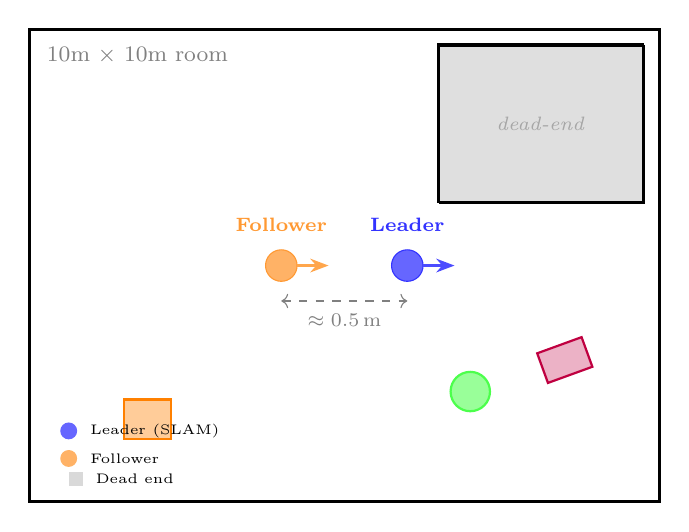
\begin{tikzpicture}[every node/.style={font=\small}]
  %% Room boundary
  \draw[very thick] (-4,-3) rectangle (4,3);
  \node[font=\footnotesize, gray, anchor=north west] at (-3.9,2.9) {10m $\times$ 10m room};

  %% Dead-end corridor (NE quadrant)
  \fill[gray!25] (1.2,0.8) rectangle (3.8,2.8);
  \draw[very thick] (1.2,0.8) -- (1.2,2.8) -- (3.8,2.8);
  \draw[very thick] (1.2,0.8) -- (3.8,0.8) -- (3.8,2.8);
  \node[font=\scriptsize, gray!70] at (2.5,1.8) {\textit{dead-end}};

  %% Obstacles
  \fill[orange!40, draw=orange, thick] (-2.8,-2.2) rectangle (-2.2,-1.7);
  \fill[green!40, draw=green!70, thick] (1.6,-1.6) circle (0.25);
  \fill[purple!30, draw=purple, thick, rotate around={20:(2.8,-1.2)}]
    (2.5,-1.4) rectangle (3.1,-1.0);

  %% Leader
  \filldraw[fill=blue!60, draw=blue!80] (0.8,0) circle (0.2);
  \draw[-{Stealth}, blue!70, thick] (1.0,0) -- (1.4,0);
  \node[blue!80, above=3pt, font=\bfseries\scriptsize] at (0.8,0.2) {Leader};

  %% Follower
  \filldraw[fill=orange!60, draw=orange!80] (-0.8,0) circle (0.2);
  \draw[-{Stealth}, orange!70, thick] (-0.6,0) -- (-0.2,0);
  \node[orange!80, above=3pt, font=\bfseries\scriptsize] at (-0.8,0.2) {Follower};

  %% Distance annotation
  \draw[<->, gray, dashed] (-0.8,-0.45) -- (0.8,-0.45);
  \node[below=1pt, gray, font=\scriptsize] at (0,-0.45) {$\approx 0.5$\,m};

  % %% Spawn markers
  % \draw[blue!40, dotted] (0.8,-0.2) -- (0.8,-0.75);
  % \node[blue!40, font=\tiny] at (0.8,-0.9) {spawn$(1, 0)$};
  % \draw[orange!40, dotted] (-0.8,-0.2) -- (-0.8,-0.75);
  % \node[orange!40, font=\tiny] at (-0.8,-0.9) {spawn$(-0.5, 0)$};

  %% Legend (inside lower-left)
  \begin{scope}[shift={(-3.5,-2.1)}]
    \filldraw[blue!60] (0,0) circle(0.1); \node[right, font=\tiny] at (0.15,0) {Leader (SLAM)};
    \filldraw[orange!60] (0,-0.35) circle(0.1); \node[right, font=\tiny] at (0.15,-0.35) {Follower};
    \fill[gray!30] (0,-0.7) rectangle (0.18,-0.52); \node[right, font=\tiny] at (0.22,-0.61) {Dead end};
  \end{scope}
\end{tikzpicture}
\caption{Top-down view of the exploration environment. The leader navigates into the
dead-end corridor (NE quadrant); the follower must coordinate to resolve the situation.}
\label{fig:world}
\end{figure}

\subsection{Edge Cases to Handle}

Real cooperative robot systems must be robust.
The following \emph{edge cases} are part of the formal specification and must be
handled by your implementation:

\begin{enumerate}[label=\textbf{EC\arabic*.}]
  \item \textbf{Follower too far.}
        The leader starts moving but the follower has not yet reached the correct
        following distance. The leader must wait while the follower approaches.
  \item \textbf{Leader hits a dead end.}
        The leader detects that all forward paths are blocked by obstacles.
        It signals the follower to back up, reverses out, and resumes exploration.
        The follower temporarily drives forward to keep the path clear.
  \item \textbf{Follower loses the leader.}
        Signal timeout or excessive distance causes the follower to lose track.
        The follower searches using the last known position;
        the leader halts and broadcasts its location until the follower recovers.
  \item \textbf{Both robots stuck (mutual wait).}
        If both robots are simultaneously waiting for the other, the system must
        eventually time out and recover — not deadlock indefinitely.
\end{enumerate}

% \subsection{Learning Objectives}

% After completing this lab, you will be able to:
% \begin{itemize}
%   \item[\cmark] Draw UML-style statecharts that model the behaviour of concurrent agents.
%   \item[\cmark] Translate statecharts into Uppaal timed automata and verify safety and liveness properties.
%   \item[\cmark] Identify and argue about deadlock freedom and livelock freedom formally.
%   \item[\cmark] Generate ROS2 Python node skeletons from a formal model and fill in the implementation.
%   \item[\cmark] Test and validate a multi-robot system in Gazebo simulation.
%   \item[\cmark] (Bonus) Deploy the validated system on real TurtleBot3 Burger hardware.
% \end{itemize}

\newpage
%% ============================================================
\section{Background: Model-Driven Engineering}
%% ============================================================

\subsection{The MDE Workflow}

In MDE, a project proceeds through a series of increasingly concrete models,
each derived from the previous one through \emph{transformations}.
Figure~\ref{fig:mde_workflow} shows the workflow for this lab.

\begin{figure}[H]
\centering
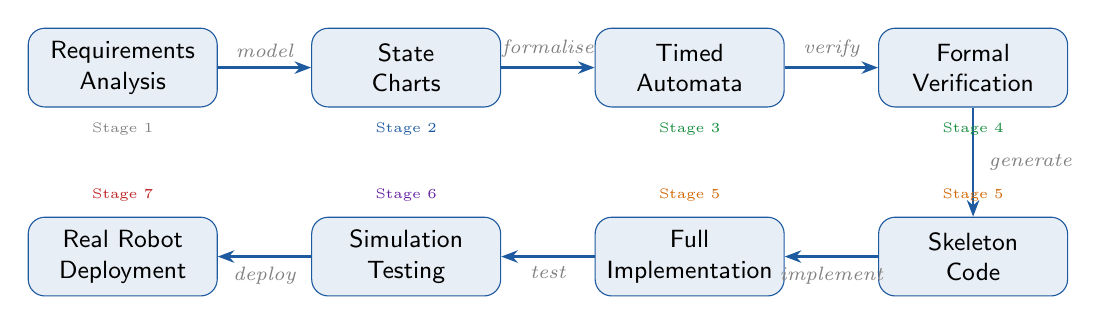
\begin{tikzpicture}[
  box/.style={draw=mdeblue, fill=mdeblue!10, rounded corners=6pt,
              minimum width=2.4cm, minimum height=1.0cm,
              text centered, font=\small\sffamily, align=center},
  arr/.style={-{Stealth[length=6pt]}, thick, mdeblue}
]
  %% Top row
  \node[box] (req) at (0,0)      {Requirements\\Analysis};
  \node[box] (sc)  at (3.6,0)    {State\\Charts};
  \node[box] (ta)  at (7.2,0)    {Timed\\Automata};
  \node[box] (ver) at (10.8,0)   {Formal\\Verification};
  %% Bottom row
  \node[box] (skel) at (10.8,-2.4) {Skeleton\\Code};
  \node[box] (impl) at (7.2,-2.4)  {Full\\Implementation};
  \node[box] (sim)  at (3.6,-2.4)  {Simulation\\Testing};
  \node[box] (hw)   at (0,-2.4)    {Real Robot\\Deployment};

  %% Top row arrows (labels above)
  \draw[arr] (req)  -- node[above, font=\scriptsize\itshape, gray]{model}     (sc);
  \draw[arr] (sc)   -- node[above, font=\scriptsize\itshape, gray]{formalise} (ta);
  \draw[arr] (ta)   -- node[above, font=\scriptsize\itshape, gray]{verify}    (ver);
  %% Vertical arrow (label to the right)
  \draw[arr] (ver)  -- node[right=2pt, font=\scriptsize\itshape, gray]{generate} (skel);
  %% Bottom row arrows (labels below)
  \draw[arr] (skel) -- node[below, font=\scriptsize\itshape, gray]{implement} (impl);
  \draw[arr] (impl) -- node[below, font=\scriptsize\itshape, gray]{test}      (sim);
  \draw[arr] (sim)  -- node[below, font=\scriptsize\itshape, gray]{deploy}    (hw);

  %% Stage labels (above for top row, below for bottom row)
  \foreach \n/\lbl/\col in {req/Stage 1/gray, sc/Stage 2/mdeblue, ta/Stage 3/mdegreen, ver/Stage 4/mdegreen}{
    \node[font=\tiny, text=\col, below=2pt] at (\n.south) {\lbl};
  }
  \foreach \n/\lbl/\col in {skel/Stage 5/mdeorange, impl/Stage 5/mdeorange, sim/Stage 6/mdepurple, hw/Stage 7/mdered}{
    \node[font=\tiny, text=\col, above=2pt] at (\n.north) {\lbl};
  }
\end{tikzpicture}
\caption{The MDE workflow followed in this lab. Each arrow represents a transformation.}
\label{fig:mde_workflow}
\end{figure}

\subsection{Tools Used}

\begin{center}
\begin{tabularx}{0.92\textwidth}{lXl}
\toprule
\textbf{Tool} & \textbf{Purpose} & \textbf{Stage} \\
\midrule
ITEMIS Create  & Graphical statechart editor (export diagram as PNG/SVG)       & 2 \\
Uppaal 5.x     & Timed automata editor + model checker (free, \url{uppaal.org}) & 3–4 \\
ROS2 Humble    & Robot operating system middleware & 5–7 \\
Gazebo Classic 11 & Physics-based simulation & 6 \\
Nav2           & Navigation stack (path planning) & 5–7 \\
slam\_toolbox  & SLAM for the leader robot & 5–7 \\
RViz2          & Visualisation of map, robots, markers & 6–7 \\
\bottomrule
\end{tabularx}
\end{center}

\subsection{Repository Structure}

The starter repository is located at \texttt{/Users/.../ros\_projects/leader\_follower/}
with the following layout:

\begin{lstlisting}[style=shellcode]
leader_follower/
  models/
    statecharts/
      leader_statechart.ysc       # Leader ITEMIS Create model (your starting point)
      follower_statechart.ysc     # Follower ITEMIS Create model
    uppaal/
      leader_follower.xml         # Uppaal model (3 templates, 14 channels)
      leader_follower.q           # Verification queries
  src/
    leader_follower_msgs/         # Custom ROS2 messages (build this FIRST)
    simulation/                   # Gazebo world, launch files, RViz config
    leader_node/
      leader_node/
        leader_node_skeleton.py   # <-- YOUR starting point (Stage 5)
        leader_node.py            # Reference solution (DO NOT peek yet!)
    follower_node/
      follower_node/
        follower_node_skeleton.py # <-- YOUR starting point (Stage 5)
        follower_node.py          # Reference solution
    visualization_node/           # Provided: visualises robots in RViz2
\end{lstlisting}

\newpage
%% ============================================================
\section{Stage 1 — Requirements Analysis}
%% ============================================================

\begin{infobox}{Goal of this Stage}
Understand the system requirements before writing any model or code.
\end{infobox}

\subsection{System Requirements}

The system must satisfy the following requirements.

\subsubsection{Functional Requirements}

\begin{enumerate}[label=\textbf{FR\arabic*.}]
  \item The leader robot shall explore the environment autonomously using SLAM.
  \item The follower robot shall maintain a distance of $0.5 \pm 0.2$\,m behind the leader.
  \item If the follower's distance exceeds 1.5\,m, the leader shall pause and wait.
  \item If the leader detects a dead end (all forward paths blocked), it shall signal
        the follower and execute a reversal manoeuvre.
  \item If the follower loses contact with the leader (no status message for $> 5$\,s),
        the follower shall execute a search procedure and the leader shall halt.
  \item Both robots shall recover from every edge case without operator intervention,
        within the time bounds specified in the timed automata model.
\end{enumerate}

\subsubsection{Safety Requirements}

\begin{enumerate}[label=\textbf{SR\arabic*.}]
  \item The system shall \emph{never} deadlock — at least one robot must always be
        able to make progress.
  \item The follower shall not drive closer than 0.2\,m to any obstacle.
  \item The maximum time spent in any waiting state shall be bounded (see Table~\ref{tab:timeouts}).
\end{enumerate}

\begin{table}[H]
\centering
\caption{State timeout bounds (encoded as clock invariants in the Uppaal model).}
\label{tab:timeouts}
\begin{tabular}{lll}
\toprule
\textbf{State} & \textbf{Robot} & \textbf{Max duration} \\
\midrule
\texttt{WAITING\_FOR\_FOLLOWER}     & Leader   & 60\,s  \\
\texttt{DEAD\_END}                  & Leader   & 15\,s  \\
\texttt{WAITING\_FOR\_LOST\_FOLLOWER} & Leader & 120\,s \\
\texttt{APPROACHING}                & Follower & 60\,s  \\
\texttt{SEARCHING\_FOR\_LEADER}     & Follower & 90\,s  \\
\bottomrule
\end{tabular}
\end{table}

\begin{Ex}{Requirements Review}
Before proceeding, answer the following questions in your lab report:
\begin{enumerate}
  \item Which requirements are \emph{safety} properties (``bad things never happen'')?
        Which are \emph{liveness} properties (``good things eventually happen'')?
  \item Describe in your own words what edge case EC4 (mutual wait) means in terms
        of robot behaviour. What would happen without the timeout bounds?
  \item List any additional edge case you think the specification is missing.
        Justify your answer.
\end{enumerate}
\end{Ex}

\newpage
%% ============================================================
\section{Stage 2 — State Machine Modelling (ITEMIS Create)}
%% ============================================================

\begin{infobox}{Goal of this Stage}
Create precise, readable statechart models for both robots.
Statecharts are the bridge between informal requirements and formal timed automata.
\end{infobox}

\subsection{Provided Models}

Open the provided ITEMIS Create projects in the ITEMIS Create IDE
(Eclipse-based; import via \texttt{File $\to$ Import $\to$ Existing Projects into Workspace}).

\medskip
\noindent\textbf{File:} \texttt{models/statecharts/leader\_statechart.ysc}

The leader statechart defines the following states and key transitions:

\begin{center}
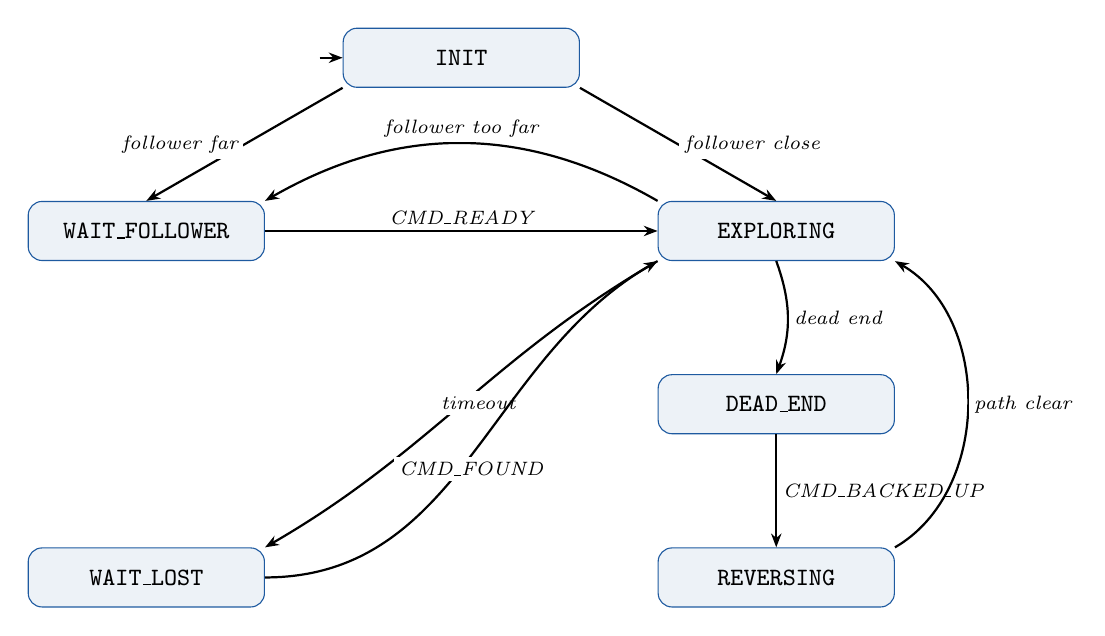
\begin{tikzpicture}[
  state/.style={draw=mdeblue, fill=mdeblue!8, rounded corners=5pt,
                minimum width=3.0cm, minimum height=0.75cm,
                text centered, font=\small\sffamily},
  arr/.style={-{Stealth[length=5pt]}, thick},
  lbl/.style={font=\scriptsize\itshape, fill=white, inner sep=2pt}
]
  %% Layout: wider spacing, three columns
  \node[state] (init) at (0,0)           {\texttt{INIT}};
  \node[state] (wff)  at (-4.0,-2.2)    {\texttt{WAIT\_FOLLOWER}};
  \node[state] (exp)  at (4.0,-2.2)     {\texttt{EXPLORING}};
  \node[state] (de)   at (4.0,-4.4)     {\texttt{DEAD\_END}};
  \node[state] (rev)  at (4.0,-6.6)     {\texttt{REVERSING}};
  \node[state] (wlf)  at (-4.0,-6.6)    {\texttt{WAIT\_LOST}};

  %% Entry arrow
  \draw[arr] (-1.8,0) -- (init);
  %% INIT transitions (angled, clear separation)
  \draw[arr] (init.south west) -- node[lbl, left]{follower far} (wff.north);
  \draw[arr] (init.south east) -- node[lbl, right]{follower close} (exp.north);
  %% WAIT_FOLLOWER --> EXPLORING
  \draw[arr] (wff.east)  -- node[lbl, above]{CMD\_READY} (exp.west);
  %% EXPLORING --> DEAD_END (bend right along right side)
  \draw[arr] (exp.south) to[bend left=20] node[lbl, right]{dead end} (de.north);
  %% EXPLORING --> WAIT_FOLLOWER (curved above the direct path to avoid crossing)
  \draw[arr] (exp.north west) to[out=150, in=30] node[lbl, above]{follower too far} (wff.north east);
  %% EXPLORING --> WAIT_LOST (long diagonal, routed via left)
  \draw[arr] (exp.south west) to[out=210, in=30] node[lbl, below, pos=0.45]{timeout} (wlf.north east);
  %% DEAD_END --> REVERSING
  \draw[arr] (de.south) -- node[lbl, right]{CMD\_BACKED\_UP} (rev.north);
  %% REVERSING --> EXPLORING (bend back up along right side)
  \draw[arr] (rev.north east) to[out=30, in=-30] node[lbl, right]{path clear} (exp.south east);
  %% WAIT_LOST --> EXPLORING
  \draw[arr] (wlf.east) to[out=0, in=-150] node[lbl, below, pos=0.5]{CMD\_FOUND} (exp.south west);
\end{tikzpicture}
\end{center}

\subsection{ITEMIS Create Notation Summary}

\begin{lstlisting}[style=xmlcode, caption={ITEMIS Create Statechart Language (SCL) syntax (excerpt).}]
// Interface declarations (in the statechart specification)
@EventDriven
interface:
    in event follower_close    // incoming event
    in event dead_end_detected
    out event CMD_DEAD_END     // outgoing event
    var dist : real = 0.0      // variable

// Transitions inside the diagram are specified as:
//   trigger [guard] / action

// Entry transition (from Entry node to INIT)
// (graphical; no textual syntax needed)

// INIT --> EXPLORING on event with guard
follower_close [dist <= 1.0] / ;   // guard in brackets

// EXPLORING --> DEAD_END on event with action
dead_end_detected / raise CMD_DEAD_END;

// Timed transition: leave state after 60 seconds
after 60s / ;
\end{lstlisting}

Notation: \texttt{trigger [guard] / action} — guards are boolean expressions
in square brackets; actions use \texttt{raise Interface.event} or variable assignments.

\begin{Ex}{Statechart Inspection and Extension}
\begin{enumerate}
  \item Export both ITEMIS Create statecharts (leader + follower) as PNG or SVG.
        Include the exported diagrams in your report.
  \item The follower statechart is missing a direct transition from
        \texttt{LEADING\_TEMPORARILY} to \texttt{SEARCHING\_FOR\_LEADER}
        for the case where the leader goes silent during the reversal manoeuvre.
        \begin{enumerate}[label=\alph*)]
          \item Add this transition to \texttt{follower\_statechart.ysc} in ITEMIS Create.
          \item Specify the guard condition and any actions on the new transition.
        \end{enumerate}
  \item Propose and add one additional state to \emph{either} robot's statechart
        that represents a scenario not yet modelled (e.g.\ battery low, sensor fault).
        Justify your choice and specify all new transitions.
  \item Identify the \emph{orthogonal region} in the follower statechart
        (communication sub-machine). What purpose does it serve?
\end{enumerate}
\end{Ex}

\newpage
%% ============================================================
\section{Stage 3 — Timed Automata (Uppaal)}
%% ============================================================

\begin{infobox}{Goal of this Stage}
Translate the statecharts into Uppaal timed automata, which allow formal verification.
The key difference from statecharts: every state can have a \emph{clock invariant}
(``this state is exited within $x$ seconds'') and transitions can have \emph{guards}
(conditions on clocks and variables).
\end{infobox}

\subsection{What is a Timed Automaton?}

A Timed Automaton (TA) extends a finite-state automaton with:
\begin{itemize}
  \item \textbf{Clocks} $x, y, \ldots \in \mathbb{R}_{\geq 0}$ — real-valued timers that increment continuously.
  \item \textbf{Clock invariants} on locations: e.g.\ $x \leq 15$ means ``leave this
        state within 15 seconds.''
  \item \textbf{Clock guards} on transitions: e.g.\ $x \geq 5$ enables a transition only
        after 5 seconds.
  \item \textbf{Resets}: $x := 0$ resets a clock on a transition.
\end{itemize}

A \textbf{network of timed automata} (NTA) is a set of TA running in parallel,
synchronising via channels: \texttt{signal!} (sender) pairs with \texttt{signal?} (receiver).

\subsection{The Provided Uppaal Model}

Open \texttt{models/uppaal/leader\_follower.xml} in Uppaal 5.x.
The model contains three templates:

\begin{center}
\begin{tabularx}{0.88\textwidth}{lX}
\toprule
\textbf{Template} & \textbf{Role} \\
\midrule
\texttt{LeaderRobot}   & States + transitions of the leader; clock \texttt{t} with invariants \\
\texttt{FollowerRobot} & States + transitions of the follower; clock \texttt{t} with invariants \\
\texttt{Environment}   & Non-deterministic event generator: obstacles, signal loss, distance changes \\
\bottomrule
\end{tabularx}
\end{center}

\noindent Global channel declarations (excerpt):

\begin{lstlisting}[style=uppaalcode, caption={Global declarations in leader\_follower.xml.}]
chan follower_ready;          // Follower -> Leader: in position
chan leader_start;            // Leader -> Follower: begin
broadcast chan dead_end_alert; // Leader -> Follower: dead end!
chan follower_backed_up;       // Follower -> Leader: backed up
chan reversal_done;            // Leader -> Follower: reversal complete
chan leader_lost_signal;       // Follower -> Leader: lost contact
chan leader_found_reply;       // Leader -> Follower: I am here
broadcast chan emergency_stop; // All -> All: halt
\end{lstlisting}

\subsection{Query Language}

Uppaal uses a subset of Computation Tree Logic (CTL):

\begin{center}
\begin{tabular}{lll}
\toprule
\textbf{Syntax} & \textbf{Reading} & \textbf{Type} \\
\midrule
\texttt{A[] p}   & $p$ always holds on all paths & safety \\
\texttt{E<> p}   & $p$ eventually holds on some path & reachability \\
\texttt{A<> p}   & $p$ eventually holds on all paths & (strong) liveness \\
\texttt{E[] p}   & $p$ always holds on some path & — \\
\texttt{p --> q} & whenever $p$, eventually $q$ (leads-to) & liveness \\
\bottomrule
\end{tabular}
\end{center}

\noindent The special predicate \texttt{deadlock} is true in a state where no transition
is enabled (even after arbitrary time passage).

\begin{Ex}{Loading and Running Queries}
\begin{enumerate}
  \item Open \texttt{leader\_follower.xml} in Uppaal. Navigate to the
        \emph{Simulator} tab and step through an execution to get a feel for
        the model.
  \item Open \texttt{leader\_follower.q} via \emph{File $\to$ Open Queries}.
        Run all 14 queries from the \emph{Verifier} tab.
  \item Record your results in the following table (fill the Expected and Result columns):
\end{enumerate}

\medskip
\begin{center}
\small
\footnotesize
\begin{tabularx}{\textwidth}{c>{\raggedright\arraybackslash}Xlcc}
\toprule
\textbf{\#} & \textbf{Query} & \textbf{Type} & \textbf{Expected} & \textbf{Result} \\
\midrule
1  & \texttt{A[] not deadlock}                                         & safety      & SAT & \hspace{1cm} \\
2  & \texttt{E<> (Leader.EXPLORING and Follower.FOLLOWING)}            & reach.      & SAT & \\
3  & \texttt{Follower.APPROACHING {-}{-}> Follower.FOLLOWING}          & liveness    & SAT & \\
4  & \texttt{Leader.DEAD\_END {-}{-}> Leader.EXPLORING}                & liveness    & SAT & \\
5  & \texttt{Follower.SEARCHING\_FOR\_LEADER {-}{-}> Follower.APPROACHING} & liveness & SAT & \\
6  & \texttt{E<> Leader.DEAD\_END}                                     & reach.      & SAT & \\
7  & \texttt{E<> Follower.LEADING\_TEMPORARILY}                        & reach.      & SAT & \\
8  & no mutual timeout (clock bound)                                   & safety      & SAT & \\
9  & \texttt{A[] (WAIT\_FOLLOWER $\Rightarrow$ t $\leq$ 60)}           & safety      & SAT & \\
10 & \texttt{A[] (SEARCHING $\Rightarrow$ t $\leq$ 90)}                & safety      & SAT & \\
11 & progress from EXPLORING                                           & liveness    & SAT & \\
12 & \texttt{A<> (Leader.EXPLORING and Follower.FOLLOWING)}            & univ.\ live. & ? & \\
13 & mutual exclusion of conflicting states                            & safety      & SAT & \\
14 & follower leading $\Rightarrow$ leader reversing/exploring         & safety      & SAT & \\
\bottomrule
\end{tabularx}
\normalsize
\end{center}
\end{Ex}

\begin{Ex}{Analysing Query 12}
Query 12 (\texttt{A<>} universal liveness) is marked with ``?'' because it may
\emph{not} be satisfied.
\begin{enumerate}
  \item Run query 12. If it fails, Uppaal will show a \emph{counter-example trace}.
        Use the simulator to step through it and identify which states are reached.
  \item Explain in your own words why \texttt{A<>} is harder to satisfy than \texttt{E<>}.
  \item The failure is caused by the \texttt{ERROR} states in both templates.
        Modify query 12 to \emph{assume} neither robot is in \texttt{ERROR}
        and re-verify. Hint: use the \texttt{imply} operator or add a guard.
  \item Add a new property of your own that is meaningful for this system
        (e.g.\ ``after a dead end, reversal completes within 30 seconds'').
        Write the query, add it to \texttt{leader\_follower.q}, and verify it.
        Explain the result.
\end{enumerate}
\end{Ex}

\begin{Ex}{Extending the Uppaal Model}
\begin{enumerate}
  \item The \texttt{Environment} template currently models distance changes
        by cycling through values 0–2 deterministically.
        Modify it so that the distance can also jump directly to 3 (LOST)
        at any time, simulating sudden signal loss.
        Re-verify the deadlock-freedom query. Does it still hold?
  \item Add a \texttt{BatteryMonitor} template that:
        \begin{itemize}
          \item maintains an integer variable \texttt{battery} (100 $\to$ 0) that
                decreases over time;
          \item sends an \texttt{emergency\_stop} broadcast when
                \texttt{battery == 0};
          \item resets when \texttt{emergency\_stop} is received
                (robot returns to dock).
        \end{itemize}
        Write at least two new queries for the extended model.
\end{enumerate}
\end{Ex}

\newpage
%% ============================================================
\section{Stage 4 — Property Verification Summary}
%% ============================================================

\begin{infobox}{Goal of this Stage}
Consolidate your verification results and argue formally about key system properties.
This stage is primarily a \emph{report-writing} stage.
\end{infobox}

\begin{Ex}{Verification Report}
Write a concise section (1–2 pages) in your lab report that:
\begin{enumerate}
  \item States the three most important properties for this system and justifies why.
  \item For each property, gives:
        \begin{itemize}
          \item The informal English description,
          \item The formal Uppaal query,
          \item The verification result (satisfied / not satisfied),
          \item A brief argument for \emph{why} it holds (or what assumption is needed).
        \end{itemize}
  \item Compares the properties verified here with what you would need for a
        \emph{safety-critical} certification (e.g.\ ISO\,26262 for automotive systems).
        What additional properties would you need to verify?
\end{enumerate}
\end{Ex}

\newpage
%% ============================================================
\section{Stage 5 — Code Skeleton and Implementation}
%% ============================================================

\begin{infobox}{Goal of this Stage}
Translate the verified formal model into executable ROS2 Python code.
You will fill in the state machine logic in the provided skeleton files.
\end{infobox}

\subsection{Architecture Overview}

The system runs as five cooperating ROS2 nodes:

\begin{figure}[H]
\centering
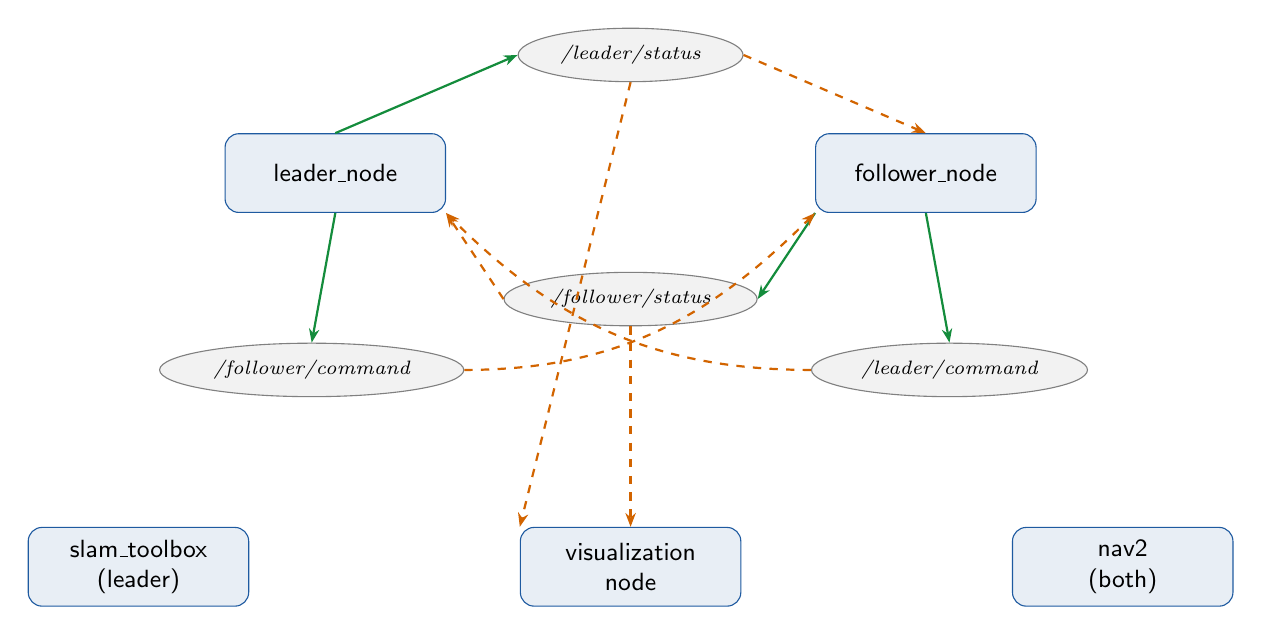
\begin{tikzpicture}[
  rosnode/.style={draw=mdeblue, fill=mdeblue!10, rounded corners=5pt,
               minimum width=2.8cm, minimum height=1.0cm, text centered,
               font=\small\sffamily, align=center},
  topic/.style={draw=gray, fill=gray!10, ellipse,
                minimum width=2.6cm, minimum height=0.55cm,
                font=\scriptsize\itshape, align=center},
  pub/.style={-{Stealth[length=5pt]}, thick, mdegreen},
  sub/.style={-{Stealth[length=5pt]}, thick, mdeorange, dashed}
]
  %% Nodes — spread out horizontally
  \node[rosnode] (ln)   at (0,4)      {leader\_node};
  \node[rosnode] (fn)   at (7.5,4)    {follower\_node};
  \node[rosnode] (vn)   at (3.75,-1)  {visualization\\node};
  \node[rosnode] (slam) at (-2.5,-1)  {slam\_toolbox\\(leader)};
  \node[rosnode] (nav)  at (10,-1)    {nav2\\(both)};

  %% Topics — clear vertical separation
  \node[topic] (ls)  at (3.75,5.5)  {/leader/status};
  \node[topic] (fs)  at (3.75,2.4)  {/follower/status};
  \node[topic] (fc)  at (-0.3,1.5)  {/follower/command};
  \node[topic] (lc)  at (7.8,1.5)   {/leader/command};

  %% /leader/status: leader publishes, follower + viz subscribe
  \draw[pub] (ln.north)  -- (ls.west);
  \draw[sub] (ls.east)   -- (fn.north);
  \draw[sub] (ls.south)  -- (vn.north west);

  %% /follower/status: follower publishes, leader + viz subscribe
  \draw[pub] (fn.south west) -- (fs.east);
  \draw[sub] (fs.west)       -- (ln.south east);
  \draw[sub] (fs.south)      -- (vn.north);

  %% /follower/command: leader publishes, follower subscribes
  \draw[pub] (ln.south)       -- (fc.north);
  \draw[sub] (fc.east)        to[out=0, in=-135] (fn.south west);

  %% /leader/command: follower publishes, leader subscribes
  \draw[pub] (fn.south)       -- (lc.north);
  \draw[sub] (lc.west)        to[out=180, in=-45] (ln.south east);
\end{tikzpicture}
\caption{ROS2 node communication graph. Green solid = publish; orange dashed = subscribe.}
\end{figure}

\subsection{Custom Messages}

Two custom message types are defined in \texttt{src/leader\_follower\_msgs/msg/}:

\begin{lstlisting}[style=pycode, caption={RobotStatus.msg — broadcast by each robot at 10\,Hz.}]
std_msgs/Header header
uint8  state          # current state enum value
string state_name     # human-readable state name
float64 x, y         # position in map frame (from odometry)
float64 heading      # yaw angle in radians
float64 distance_to_other  # Euclidean distance to other robot

uint8 STATE_INIT=0    uint8 STATE_EXPLORING=2   uint8 STATE_DEAD_END=5
uint8 STATE_REVERSING=6     uint8 STATE_WAITING_FOR_LOST_FOLLOWER=11
uint8 STATE_FOLLOWING=3     uint8 STATE_APPROACHING=4
# ...
\end{lstlisting}

\begin{lstlisting}[style=pycode, caption={CoordinationCommand.msg — sent on state transitions.}]
std_msgs/Header header
uint8  command   # one of the CMD_* constants below
string data      # optional payload (e.g., "x,y" for I_AM_HERE)

uint8 CMD_READY=0   uint8 CMD_DEAD_END=7   uint8 CMD_BACKED_UP=11
uint8 CMD_RESUME=2  uint8 CMD_LOST_YOU=9   uint8 CMD_I_AM_HERE=6
# ...
\end{lstlisting}

\subsection{Building the Workspace}

\begin{lstlisting}[style=shellcode]
cd ~/ros_projects/leader_follower
export TURTLEBOT3_MODEL=burger
export RMW_IMPLEMENTATION=rmw_cyclonedds_cpp
colcon build --symlink-install
source install/setup.bash
\end{lstlisting}

\begin{warnbox}{Important}
Always build \texttt{leader\_follower\_msgs} first (colcon handles this automatically
via dependency resolution). If you encounter import errors, run
\texttt{colcon build --packages-select leader\_follower\_msgs} first.
\end{warnbox}

\subsection{Skeleton File Structure}

Open \texttt{src/leader\_node/leader\_node/leader\_node\_skeleton.py}.
Every \texttt{\# TODO} comment corresponds to a state handler that you must implement.
The helper methods (LiDAR sector analysis, \texttt{\_stop()}, \texttt{\_transition\_to()},
\texttt{\_send\_command\_to\_follower()}) are fully provided — use them.

\begin{Ex}{Implement the Leader Node}
Fill in the following methods in \texttt{leader\_node\_skeleton.py}:
\begin{enumerate}
  \item \textbf{\texttt{\_handle\_init()}} — Check if follower status has been received;
        transition to \texttt{EXPLORING} (close) or \texttt{WAITING\_FOR\_FOLLOWER} (far).
  \item \textbf{\texttt{\_handle\_exploring()}} — This is the core handler.
        Implement the following priority chain:
        \begin{enumerate}[label=\roman*.]
          \item If follower is not connected (\texttt{\_follower\_is\_connected()} returns False)
                → transition to \texttt{WAITING\_FOR\_LOST\_FOLLOWER}.
          \item If \texttt{follower\_distance > FOLLOW\_DISTANCE\_FAR}
                → stop robot, transition to \texttt{WAITING\_FOR\_FOLLOWER}.
          \item If \texttt{\_is\_dead\_end()} returns True for
                \texttt{DEAD\_END\_CONFIRM\_SCANS} consecutive calls
                → send \texttt{CMD\_DEAD\_END}, transition to \texttt{DEAD\_END}.
          \item Otherwise → publish a forward \texttt{Twist}
                (\texttt{linear.x = EXPLORE\_LINEAR}).
        \end{enumerate}
  \item \textbf{\texttt{\_handle\_dead\_end()}} — Stop robot.
        Re-broadcast \texttt{CMD\_DEAD\_END} every \texttt{DEAD\_END\_BROADCAST\_INTERVAL}
        seconds. When \texttt{self.dead\_end\_ack\_received} is True (set by the callback),
        transition to \texttt{REVERSING}.
        If \texttt{\_seconds\_in\_state() > DEAD\_END\_WAIT\_TIMEOUT},
        force transition to \texttt{REVERSING}.
  \item \textbf{\texttt{\_handle\_reversing()}} — Publish a backward Twist
        (\texttt{linear.x = LINEAR\_REVERSE\_SPEED}).
        When the forward sector minimum range exceeds
        \texttt{REVERSAL\_CLEAR\_RANGE}, stop, send \texttt{CMD\_RESUME},
        and transition to \texttt{EXPLORING}.
  \item \textbf{\texttt{\_on\_follower\_ready()}},
        \textbf{\texttt{\_on\_follower\_lost()}},
        \textbf{\texttt{\_on\_follower\_found()}} — Event handlers called by the
        command callback. Implement the state transitions for each event.
\end{enumerate}
\end{Ex}

\begin{Ex}{Implement the Follower Node}
Fill in the following methods in \texttt{follower\_node\_skeleton.py}:
\begin{enumerate}
  \item \textbf{\texttt{\_handle\_init()}} — Wait for first leader status message;
        transition to \texttt{APPROACHING}.
  \item \textbf{\texttt{\_handle\_approaching()}} — Drive toward a point
        \texttt{TARGET\_DISTANCE} behind the leader's published pose.
        Use the provided \texttt{\_compute\_approach\_goal()} to get the target position.
        Transition to \texttt{FOLLOWING} (sending \texttt{CMD\_READY}) when
        \texttt{leader\_distance} $\leq$ \texttt{APPROACH\_THRESHOLD}.
  \item \textbf{\texttt{\_handle\_following()}} — Implement the proportional controller:
        \[
          v = K_{p,v} \cdot (d - d^*), \qquad
          \omega = K_{p,\omega} \cdot \beta
        \]
        where $d$ is \texttt{self.leader\_distance},
        $d^* = 0.5$\,m (\texttt{TARGET\_DISTANCE}),
        and $\beta$ is \texttt{self.leader\_bearing}.
        Clamp $v \in [-v_{\max}, v_{\max}]$ and $\omega \in [-\omega_{\max}, \omega_{\max}]$.
        Apply the safety stop: if the forward LiDAR minimum is $< 0.20$\,m, set $v = 0$.
  \item \textbf{\texttt{\_handle\_backing\_up()}} — Drive backward at
        \texttt{BACKUP\_SPEED}. Track distance backed up using the current pose
        relative to \texttt{self.backup\_start\_x}, \texttt{self.backup\_start\_y}.
        When \texttt{distance\_backed\_up} $\geq$ \texttt{BACKUP\_DISTANCE},
        send \texttt{CMD\_BACKED\_UP} and transition to \texttt{LEADING\_TEMPORARILY}.
  \item \textbf{\texttt{\_handle\_searching()}} — Implement at least Phase 0 of the
        search algorithm (navigate to \texttt{last\_known\_leader\_x/y}).
        The heartbeat timer broadcasts \texttt{CMD\_LOST\_YOU} automatically.
        Transition to \texttt{APPROACHING} when a new leader status is received
        (this is already wired in \texttt{\_leader\_status\_callback}).
\end{enumerate}
\end{Ex}

\newpage
%% ============================================================
\section{Stage 6 — Simulation Testing (Gazebo)}
%% ============================================================

\begin{infobox}{Goal of this Stage}
Validate your implementation in the Gazebo simulation environment before
touching real hardware.
\end{infobox}

\subsection{Launching the Simulation}

\begin{lstlisting}[style=shellcode]
# Terminal 1: start simulation (Gazebo + Nav2 + SLAM + all nodes)
source install/setup.bash
ros2 launch simulation simulation.launch.py

# Terminal 2: monitor robot states
ros2 topic echo /leader/status --field state_name
ros2 topic echo /follower/status --field state_name

# Terminal 3: watch coordination commands
ros2 topic echo /follower/command
ros2 topic echo /leader/command
\end{lstlisting}

\subsection{Expected Startup Sequence}

\begin{enumerate}
  \item Gazebo loads \texttt{exploration\_world.world}; both robots spawn.
  \item Leader enters \texttt{INIT}, follower enters \texttt{INIT}.
  \item Follower transitions to \texttt{APPROACHING}, drives toward leader.
  \item Follower sends \texttt{CMD\_READY}; leader transitions to \texttt{EXPLORING}.
  \item Both enter cooperative mode: \texttt{EXPLORING} / \texttt{FOLLOWING}.
  \item Leader navigates into the dead-end corridor (NE quadrant).
  \item Leader detects dead end, sends \texttt{CMD\_DEAD\_END}.
  \item Follower transitions to \texttt{BACKING\_UP}, then \texttt{LEADING\_TEMPORARILY}.
  \item Leader reverses; clears the corridor; sends \texttt{CMD\_RESUME}.
  \item Both return to \texttt{EXPLORING} / \texttt{FOLLOWING}.
\end{enumerate}

\begin{Ex}{Observe and Document Normal Operation}
\begin{enumerate}
  \item Launch the simulation. Take a screenshot of RViz2 showing both robots
        and the growing SLAM map. Include it in your report.
  \item Record a sequence of state transitions from the terminal output.
        Do they match the expected startup sequence above?
  \item Measure the time from simulation start until both robots first reach
        cooperative mode (\texttt{EXPLORING}/\texttt{FOLLOWING}).
        Compare with the timeout bounds in Table~\ref{tab:timeouts}.
\end{enumerate}
\end{Ex}

\begin{Ex}{Test Edge Case EC2: Dead End Recovery}
\begin{enumerate}
  \item Wait until the leader naturally navigates into the dead-end corridor,
        \emph{or} use teleop to manually drive the leader into the corridor:
\begin{lstlisting}[style=shellcode]
ros2 run turtlebot3_teleop teleop_keyboard \
  --ros-args --remap /cmd_vel:=/leader/cmd_vel
\end{lstlisting}
  \item Observe the state transitions in both robots. Record the exact sequence
        of \texttt{state\_name} values published on \texttt{/leader/status}
        and \texttt{/follower/status}.
  \item Does the dead-end recovery protocol complete within the timeout
        specified in Table~\ref{tab:timeouts}? Time it.
  \item Take a screenshot of RViz2 showing the connection line colour change
        during recovery (orange = dead-end recovery in progress).
\end{enumerate}
\end{Ex}

\begin{Ex}{Test Edge Case EC3: Follower Lost}
\begin{enumerate}
  \item While both robots are in cooperative mode, kill the follower node:
\begin{lstlisting}[style=shellcode]
# Find the follower node's PID and kill it
ros2 node list
kill $(ros2 node info /follower/follower_node | grep Pid | awk '{print $2}')
# Or simply Ctrl+C in the terminal running follower_node
\end{lstlisting}
  \item Observe: the leader should transition to \texttt{WAITING\_FOR\_LOST\_FOLLOWER}
        within 5 seconds and begin broadcasting \texttt{CMD\_I\_AM\_HERE}.
  \item Restart the follower node:
\begin{lstlisting}[style=shellcode]
ros2 run follower_node follower_node
\end{lstlisting}
  \item Verify that the follower re-enters \texttt{APPROACHING} → \texttt{FOLLOWING}
        and the leader resumes \texttt{EXPLORING}.
  \item Document the recovery time (seconds from follower restart to cooperative mode).
\end{enumerate}
\end{Ex}

\begin{Ex}{Tuning the Controller (Advanced)}
The follower's proportional controller gains are defined as constants at the top
of \texttt{follower\_node.py}:
\begin{lstlisting}[style=pycode]
KP_LINEAR  = 0.35   # linear velocity proportional gain
KP_ANGULAR = 0.90   # angular velocity proportional gain
TARGET_DISTANCE = 0.50  # desired gap (meters)
\end{lstlisting}
\begin{enumerate}
  \item What happens if \texttt{KP\_LINEAR} is too large? Too small? Test both.
  \item What happens if \texttt{TARGET\_DISTANCE} is set to 0.2\,m?
        Does the safety stop activate? Why?
  \item Find a combination of gains that minimises overshoot while maintaining
        smooth following. Plot the distance over time (use \texttt{ros2 topic echo}
        and record to CSV, then plot in Python/Matlab).
\end{enumerate}
\end{Ex}

\newpage
%% ============================================================
\section{Stage 7 — Real Robot Deployment (Bonus)}
%% ============================================================

\begin{infobox}{Goal of this Stage}
Deploy the validated simulation code on real TurtleBot3 Burger hardware.
\textbf{This stage is optional} but strongly recommended for full marks.
\end{infobox}

\begin{warnbox}{Hardware Safety Rules}
\begin{itemize}
  \item Always keep a hand close to the e-stop button.
  \item Run first tests in a large, clear space with no people nearby.
  \item Ensure both robots have at least 50\,\% battery before starting.
  \item Set \texttt{MAX\_LINEAR\_VEL = 0.10} for first tests (half the default).
\end{itemize}
\end{warnbox}

\subsection{Network Setup}

Both robots and the workstation must share the same ROS2 DDS domain:

\begin{lstlisting}[style=shellcode]
# On ALL devices (workstation, leader Pi, follower Pi):
export ROS_DOMAIN_ID=42
export RMW_IMPLEMENTATION=rmw_cyclonedds_cpp

# Verify discovery:
ros2 node list   # should show nodes from all devices
\end{lstlisting}

\subsection{Per-Robot Bring-Up}

\begin{lstlisting}[style=shellcode]
# On Leader Raspberry Pi:
export TURTLEBOT3_MODEL=burger
ros2 launch turtlebot3_bringup robot.launch.py

# On Follower Raspberry Pi:
export TURTLEBOT3_MODEL=burger
ros2 launch turtlebot3_bringup robot.launch.py

# On Workstation:
ros2 launch simulation real_robot.launch.py
\end{lstlisting}

\begin{Ex}{Real Robot Validation}
\begin{enumerate}
  \item Verify that \texttt{ros2 topic list} shows \texttt{/leader/scan},
        \texttt{/follower/scan}, \texttt{/leader/odom}, and \texttt{/follower/odom}
        on the workstation.
  \item Place the robots in the correct start positions (0.5\,m apart, facing the
        same direction). Observe the initial approach sequence.
  \item If the follower oscillates (overshoot), reduce \texttt{KP\_LINEAR}.
        If it is too slow to track, increase it.
  \item Demonstrate the dead-end recovery by placing a large box in front of
        the leader while both robots are in cooperative mode.
  \item Record a video of the full demo (initial approach + exploration +
        at least one edge case recovery). Submit alongside your report.
\end{enumerate}
\end{Ex}

\newpage
%% ============================================================
\section{Deliverables and Assessment}
%% ============================================================

\subsection{Deliverables}

Submit a single ZIP archive containing:

\begin{enumerate}
  \item \textbf{Lab Report} (PDF, max 15 pages) structured as follows:
        \begin{itemize}
          \item Stage 1: Requirement classification table + EC analysis
          \item Stage 2: Rendered statecharts (original + your modifications)
          \item Stage 3–4: Verification table + property arguments
          \item Stage 5: Code diff (only your changes to the skeleton files)
          \item Stage 6: Screenshots, state transition logs, edge case results
          \item (Stage 7): Video link or attached MP4
        \end{itemize}
  \item \textbf{Modified model files:}
        \texttt{leader\_statechart.ysc},
        \texttt{follower\_statechart.ysc},\\
        \texttt{leader\_follower.xml},
        \texttt{leader\_follower.q}
  \item \textbf{Implemented node files:}
        \texttt{leader\_node\_skeleton.py},
        \texttt{follower\_node\_skeleton.py}\\
        (renamed to \texttt{leader\_node\_impl.py}, \texttt{follower\_node\_impl.py})
\end{enumerate}

\subsection{Assessment Rubric}

\begin{center}
\footnotesize
\begin{tabularx}{\textwidth}{XXr@{\hspace{8pt}}r}
\toprule
\textbf{Criterion} & \textbf{Evidence} & \textbf{Weight} & \textbf{Max pts} \\
\midrule
\textbf{Stage 1}: Req.\ analysis quality
  & Report: classification, EC4 explanation
  & 10\,\% & 10 \\
\addlinespace
\textbf{Stage 2}: Statechart correctness
  & Rendered diagrams, added transition + state
  & 15\,\% & 15 \\
\addlinespace
\textbf{Stage 3}: Uppaal query results
  & Completed verification table, correct results
  & 15\,\% & 15 \\
\addlinespace
\textbf{Stage 4}: Property arguments
  & Written justifications for top-3 properties
  & 10\,\% & 10 \\
\addlinespace
\textbf{Stage 5a}: Leader implementation
  & All 5 handler methods correct
  & 15\,\% & 15 \\
\addlinespace
\textbf{Stage 5b}: Follower implementation
  & All 5 handler methods correct
  & 15\,\% & 15 \\
\addlinespace
\textbf{Stage 6}: Simulation validation
  & Screenshots, state logs, edge case demos
  & 10\,\% & 10 \\
\addlinespace
\textbf{Stage 6 (adv.)}: Controller tuning
  & Distance plot, gain analysis
  & 5\,\% & 5 \\
\addlinespace
\textbf{Stage 7} (bonus): Real robot demo
  & Video showing all edge cases on hardware
  & +15\,\% & 15 \\
\midrule
\textbf{Total (without bonus)} & & 100\,\% & 100 \\
\textbf{Total (with bonus)}    & & 115\,\% & 115 \\
\bottomrule
\end{tabularx}
\normalsize
\end{center}

\bigskip
\begin{infobox}{Academic Integrity}
You may discuss concepts and debugging strategies with other groups,
but all model files, code, and written analysis must be your own work.
Any use of AI code-generation tools must be declared and the generated
portions clearly identified. Undeclared AI-generated code will be
treated as plagiarism.
\end{infobox}

\newpage
%% ============================================================
\section*{Appendix A — Uppaal Quick Reference}
\addcontentsline{toc}{section}{Appendix A — Uppaal Quick Reference}
%% ============================================================

\subsection*{A.1 Location Types}

\begin{center}
\begin{tabular}{lp{10cm}}
\toprule
\textbf{Type} & \textbf{Meaning} \\
\midrule
Normal      & Standard location; time may pass. \\
Initial     & Marked with a double circle; starting location. \\
Committed   & Marked with \texttt{C}; no time may pass; must take a transition immediately. \\
Urgent      & Marked with \texttt{U}; no time may pass, but can be pre-empted by other automata. \\
\bottomrule
\end{tabular}
\end{center}

\subsection*{A.2 Transition Labels}

Each edge can carry up to four labels (all optional):

\begin{center}
\begin{tabular}{lll}
\toprule
\textbf{Label} & \textbf{Example} & \textbf{Meaning} \\
\midrule
Select     & \texttt{i: int[0,3]}       & Non-deterministic binding \\
Guard      & \texttt{x >= 5}            & Condition on clocks/variables \\
Synchronisation & \texttt{signal!} / \texttt{signal?} & Send/receive on channel \\
Update     & \texttt{x = 0, count++}    & Side effects on transition \\
\bottomrule
\end{tabular}
\end{center}

\subsection*{A.3 Query Operators Cheat Sheet}

\begin{lstlisting}[style=uppaalcode]
A[] not deadlock                      // Safety: deadlock freedom
A[] P.safe_state imply x <= 10       // Clock bound invariant
E<> P.goal_state                     // Reachability
A<> P.goal_state                     // Universal liveness
P.state1 --> P.state2                // Leads-to (liveness)
A[] not (P.s1 and Q.s2)              // Mutual exclusion
\end{lstlisting}

\subsection*{A.4 Commonly Used Clock Patterns}

\begin{lstlisting}[style=uppaalcode]
// Pattern: time-bounded state (add invariant to location)
// Location "WAITING" has invariant: t <= 60
// Reset clock on entry:
trans S_PREV -> WAITING { update: t = 0 }
// Force exit after timeout:
trans WAITING -> ERROR { guard: t >= 60 }

// Pattern: periodic re-broadcast every N seconds
trans IDLE -> SEND  { guard: t >= N; update: t = 0 }
trans SEND  -> IDLE { update: action() }
\end{lstlisting}

%% ============================================================
\section*{Appendix B — ROS2 Debugging Commands}
\addcontentsline{toc}{section}{Appendix B — ROS2 Debugging Commands}
%% ============================================================

\begin{lstlisting}[style=shellcode]
# List all active nodes
ros2 node list

# Show all topics with types
ros2 topic list -t

# Monitor state transitions (10 Hz)
ros2 topic echo /leader/status --field state_name
ros2 topic echo /follower/status --field state_name

# Record a bag for later analysis
ros2 bag record /leader/status /follower/status \
  /leader/command /follower/command /leader/scan /follower/scan

# Check node graph
ros2 run rqt_graph rqt_graph

# Manual dead-end test (teleop leader into corridor)
ros2 run turtlebot3_teleop teleop_keyboard \
  --ros-args --remap /cmd_vel:=/leader/cmd_vel

# Verify Nav2 is running
ros2 action list
# Should include: /leader/navigate_to_pose, /follower/navigate_to_pose

# Check transform tree
ros2 run tf2_tools view_frames
\end{lstlisting}

%% ============================================================
\section*{Appendix C — Key Parameters Reference}
\addcontentsline{toc}{section}{Appendix C — Key Parameters Reference}
%% ============================================================

\begin{center}
\begin{tabularx}{0.96\textwidth}{lXll}
\toprule
\textbf{Parameter} & \textbf{Meaning} & \textbf{Default} & \textbf{File} \\
\midrule
\texttt{TARGET\_DISTANCE}        & Ideal follower-to-leader gap        & 0.50\,m & \texttt{follower\_node.py} \\
\texttt{APPROACH\_THRESHOLD}     & Close enough → switch to FOLLOWING  & 0.70\,m & \texttt{follower\_node.py} \\
\texttt{FAR\_THRESHOLD}          & Too far → re-approach               & 1.50\,m & both \\
\texttt{DEAD\_END\_RANGE}        & LiDAR range = blocked               & 0.40\,m & \texttt{leader\_node.py} \\
\texttt{REVERSAL\_CLEAR\_RANGE}  & Forward clear → stop reversing      & 0.80\,m & \texttt{leader\_node.py} \\
\texttt{BACKUP\_DISTANCE}        & Follower reversal depth             & 1.50\,m & \texttt{follower\_node.py} \\
\texttt{KP\_LINEAR}              & Following linear gain               & 0.35    & \texttt{follower\_node.py} \\
\texttt{KP\_ANGULAR}             & Following angular gain              & 0.90    & \texttt{follower\_node.py} \\
\texttt{FOLLOWER\_TIMEOUT}       & No msg → lost (leader side)         & 5.0\,s  & \texttt{leader\_node.py} \\
\texttt{LEADER\_TIMEOUT}         & No msg → lost (follower side)       & 5.0\,s  & \texttt{follower\_node.py} \\
\texttt{DEAD\_END\_CONFIRM\_SCANS} & Scans to confirm dead end         & 3       & \texttt{leader\_node.py} \\
\texttt{SEARCH\_TIMEOUT}         & Max search time                     & 90.0\,s & \texttt{follower\_node.py} \\
\bottomrule
\end{tabularx}
\end{center}

\end{document}
